\chapter{Conceptual Design}
\label{chap:conceptual-design}
Building on the software design of the first prototype presented in section \ref{sec:prototype-design} and the insights gained in section \ref{sec:prototype-insights}, two design concepts were worked out. The following sections will detail components and principles of both concepts.

\section{Design \#1: Monolithic Proxy Application}
\label{sec:design-1}
This design concept is based on the general ideas presented in section \ref{sec:prototype-design} (e.g. state-machines, network stacks and pipes) and employs a basic architecture shown in figure \ref{fig:component-view-1}.
\begin{figure}[h]
    \centering
    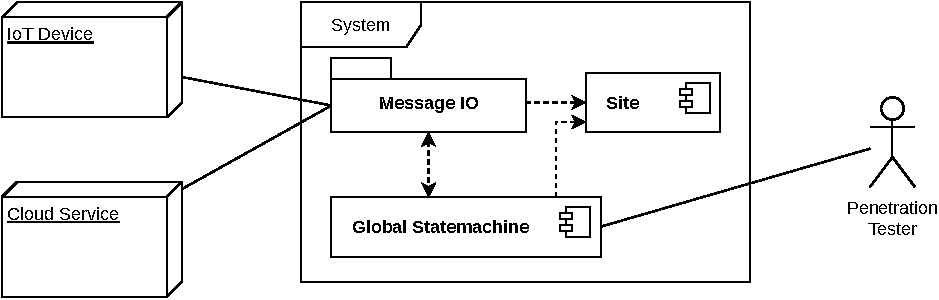
\includegraphics[width=12cm]{img/ch05/component-view-1.pdf}
    \captionof{figure}{High-level component diagram of the proxy application concept}
    \label{fig:component-view-1}
\end{figure}
\subsection{High-level Overview}
As discussed in the previous chapter, the requirement \enquote{F2 Network Stacks} introduces the need for dynamically initialized objects which in this concept is implemented by making use of the abstract factory pattern in the \enquote{Site} component (depicted in figure \ref{fig:site-factory}). This component allows for registering \emph{Factories} that are used to initialize objects. Similar to the implementation in the first prototype, factories initialize objects using metadata supplied from a configuration file.\\
\begin{figure}[H]
    \centering
    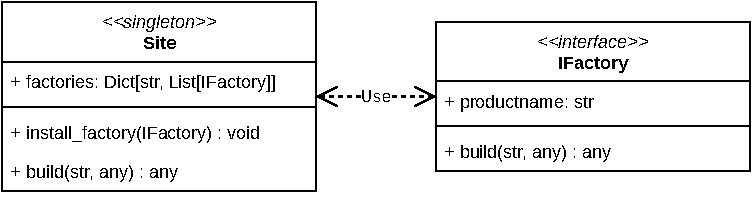
\includegraphics[width=12cm]{img/ch05/site-factory.pdf}
    \captionof{figure}{A simple variation of the abstract factory pattern. Contrary to the design of the first prototype in section \ref{sec:prototype-design}, this variation does not specify the abstract type of the products that are built as return types but as part of the meta data used for object creation.}
    \label{fig:site-factory}
\end{figure}
Communication with other systems is encapsulated into the \enquote{Message IO}-package shown in figure \ref{fig:component-view-2}. Applications that are tested by penetration testers are connected to sockets provided by the \enquote{Gateway} component and temporarily stored in a message queue to be processed by the network stacks organized by the \enquote{Global Statemachine}. Similar to the \enquote{Server} interface used in the first prototype, gateways provide means of communicating with external systems and receiving and sending messages. They are highly abstract and meant to be used for implementing interfaces for any kind of communication protocols and technologies, such as \ac{IP}-based \ac{TCP} and \ac{UDP} communication but also other protocols such as USB, Bluetooth, ZigBee or KNX.
\begin{figure}[h]
    \centering
    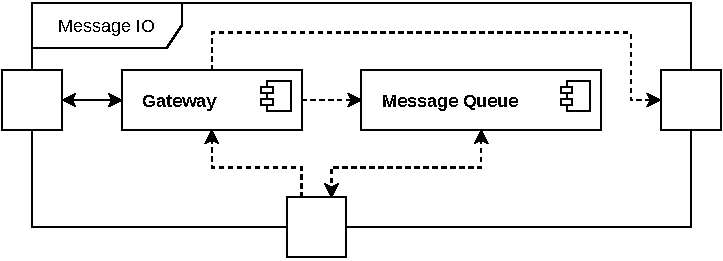
\includegraphics[width=12cm]{img/ch05/component-view-2-messageio.pdf}
    \captionof{figure}{The \enquote{Message IO}-package. The white boxes indicate ports for communication with outside components.}
    \label{fig:component-view-2}
\end{figure}
It should be noted that the static view of the design is rather simple due to its dynamic runtime behaviour: many instances and relationships are only instantiated at runtime and not pre-determined. A schematic representation of the dynamic structure and interweaving of state-machines, network stacks and pipes (in this concept called a \enquote{\emph{pipeline}}) is shown in figure \ref{fig:pipeline}.
\begin{figure}[h]
    \centering
    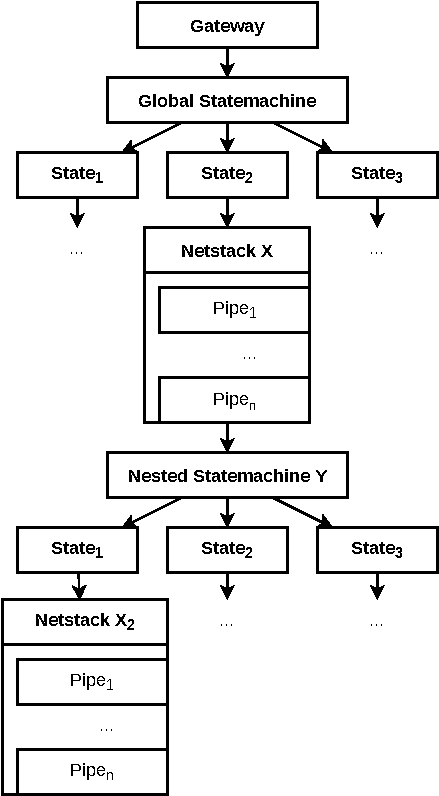
\includegraphics[height=12cm]{img/ch05/pipeline.pdf}
    \captionof{figure}{An abstract representation of the runtime hierarchy of nested \acp{FSM} and network stacks. The active states of the \acp{FSM} determine which network stacks are used, resulting in a chain of \acp{FSM} and network stacks, referred to as a \enquote{pipeline}.}
    \label{fig:pipeline}
\end{figure}This figure highlights a series of active state-machines and network stacks which together constitute the active pipeline. \\
\begin{figure}[h!]
    \centering
    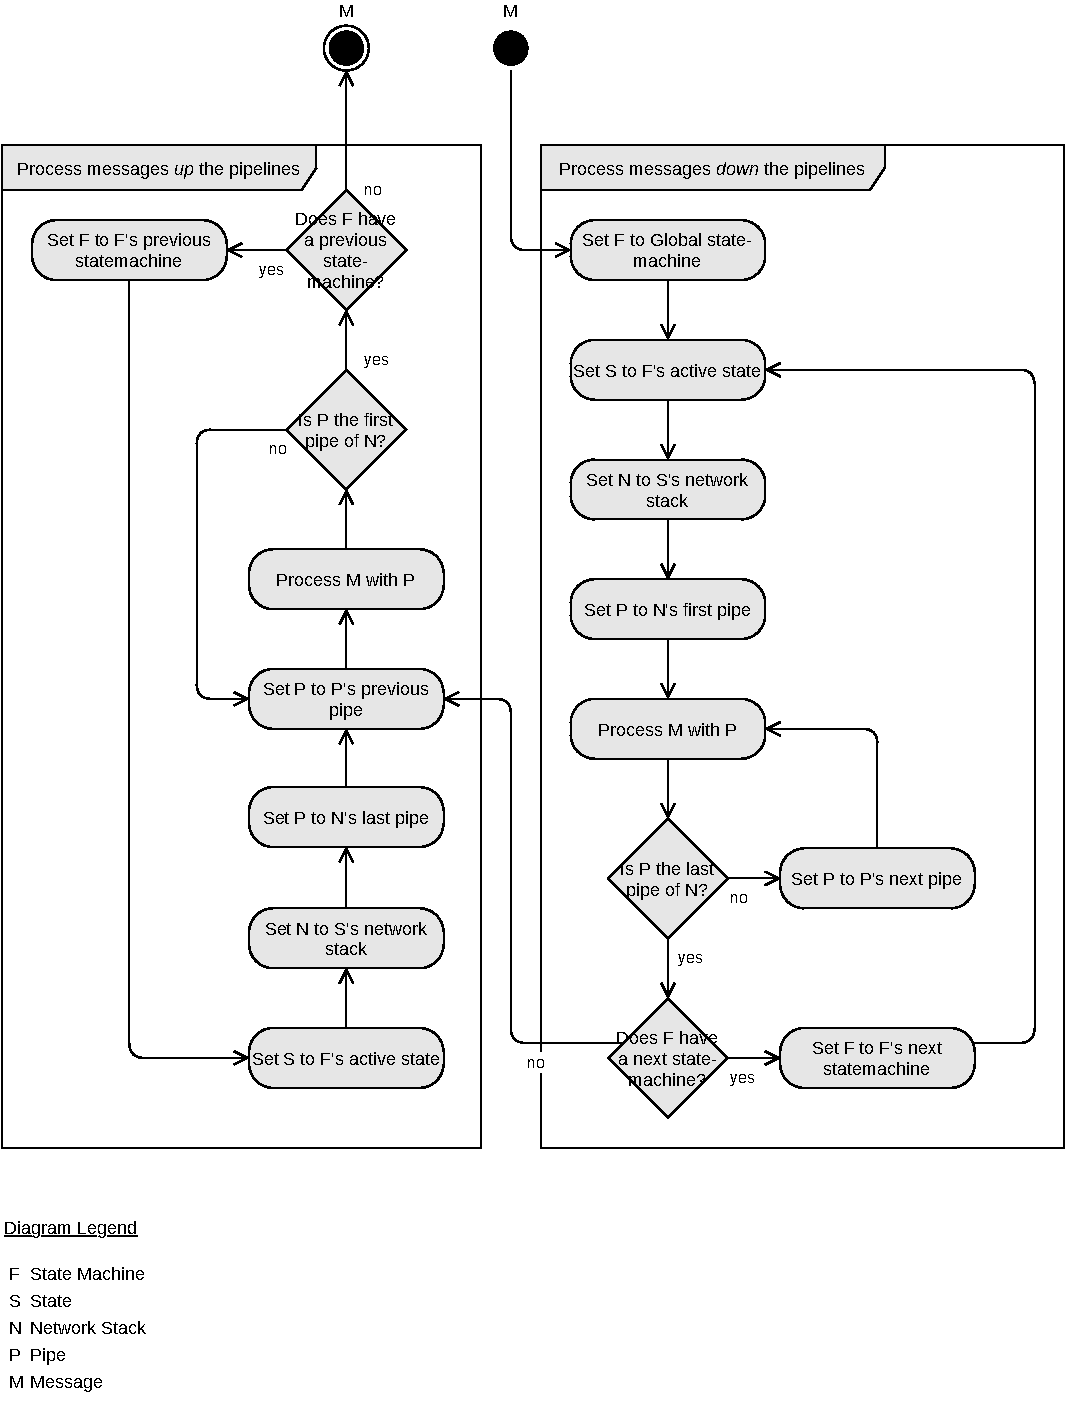
\includegraphics[width=14cm]{img/ch05/activity-nested-fsms.pdf}
    \captionof{figure}{Message processing through an architecture of nested \acp{FSM} and network stacks}
    \label{fig:activity-fsms}
\end{figure}
Figure \ref{fig:activity-fsms} illustrates the recursive nature of this concept processing (dequeued) messages:
\begin{enumerate}
    \item A state-machine $F$ (initialized with the global state-machine instance) relays messages $M$ through its active state $S$'s network stack instance $N$.
    \item In $N$, all of its pipes $P$ process $M$ until the end of $N$ is reached ($P$ does not hold a reference to a succeeding pipe instance). If $F$ holds a reference to a succeeding \ac{FSM}, $F$ is set to this reference and the process continues from step $1$.
    \item If $N$ does not hold a reference to a nested \ac{FSM}, the end of the network stack is reached and the direction of traversing the network stack is reversed.
    \item $P$ is set to $N$'s last pipe instance and $M$ is processed by $P$ until the start of $N$ is reached (i.e. $P$ does not hold a reference to a preceding pipe instance). If $F$ holds a reference to a preceding \ac{FSM} instance, $F$ is set to this reference, $N$ is set to $F$'s network stack reference and the process continues from step $4$.
    \item If $N$ does not hold a reference to a preceding \ac{FSM}, the beginning of the whole pipeline is reached and $F$ is the global state-machine.
\end{enumerate}

\begin{figure}[h]
    \centering
    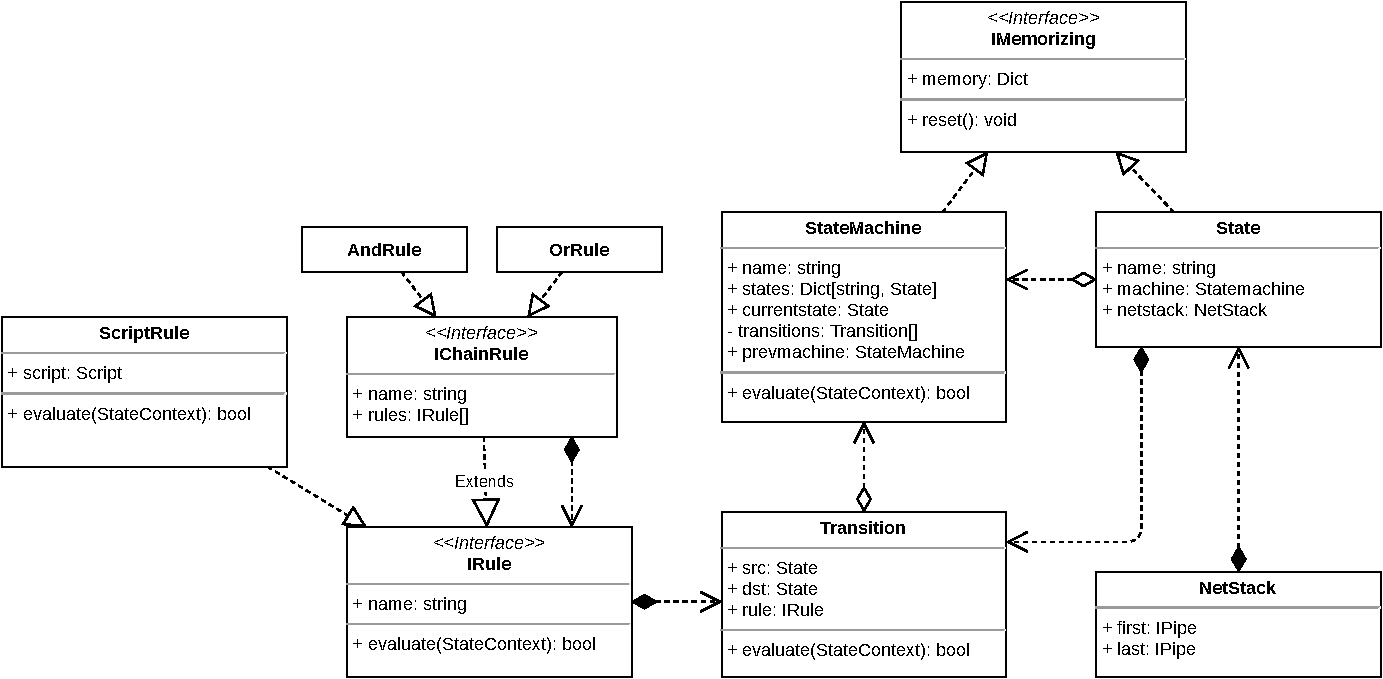
\includegraphics[width=14cm]{img/ch05/classes-1-fsm-rules-netstack.pdf}
    \captionof{figure}{\emph{StateMachines} used rules to determine whether state changes should take place. \emph{IChainRules}, \emph{AndRules} and \emph{OrRules} allowed to combine multiple rules and provided a way to specify logic using $OR$ and $AND$ operators.}
    \label{fig:classes-1-fsm-rules-netstack}
\end{figure}
\subsection{State-Machines} The classes related to the state-machine component are shown in figure \ref{fig:classes-1-fsm-rules-netstack}: \emph{StateMachines} hold a set of \emph{States} and \emph{Transitions}. In order to change states, state-machines evaluate a context by checking each of their transitions for whether their conditions for transition are met or not. This context is an aggregation of the \emph{memory} of each state-machine and their active states in the active pipeline. Transitions are defined by a source state, destination state and an \emph{IRule} that evaluates a given context. Rules can be concatenated with logical $AND$ or $OR$ operators and are designed to be scripts that operate on the given context. This allows the creation of nested rules such as the following one:
\begin{align*}
    \mathbf{changeToWS}(c) & = \mathbf{AND}(\mathbf{clientUpgrade}(c), \mathbf{serverUpgrade}(c))
\end{align*}
In this example, a transition with the above rule would evaluate to $true$ and trigger a state transition in a state-machine when the aggregated memory $c$ of all state-machines and their active states of the active pipeline indicated that an \ac{HTTP} request was detected that requested an upgrade to the \ac{WS} protocol (for instance, $clientUpgrade$ would look for an entry $clientUpgradeRequested$ in $c$ and evaluate its contents) and that an \ac{HTTP} response was detected that confirmed the upgrade request. This would allow a state-machine to detect upgrades of \ac{HTTP} communication to the \ac{WS} protocol.\\
States hold a \enquote{NetStack} which in turn encapsulate a series of connected pipes, holding references to this series' first and last elements.
\begin{figure}[h]
    \centering
    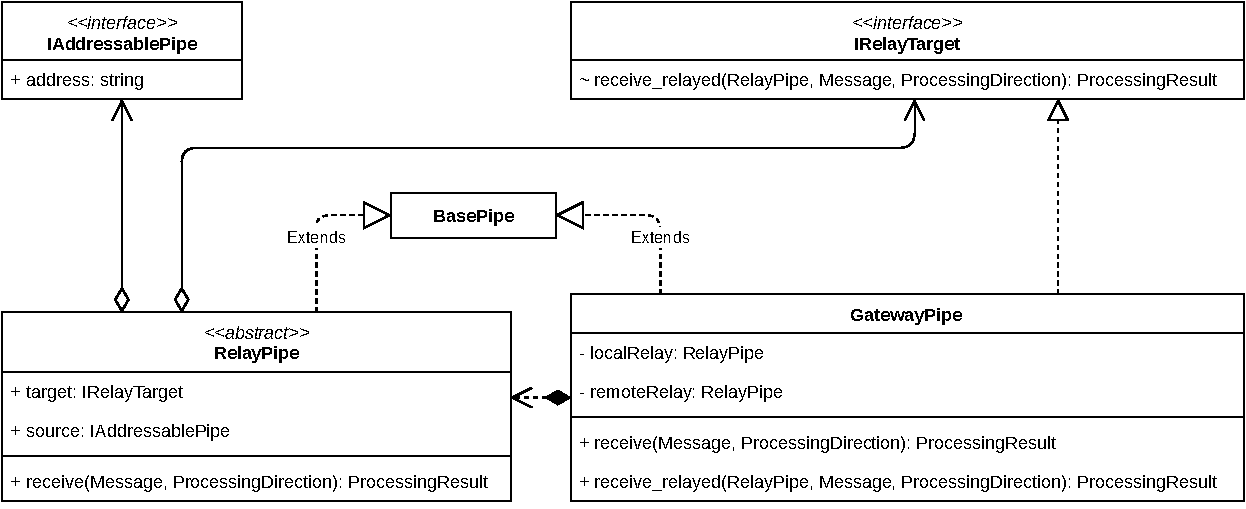
\includegraphics[width=14cm]{img/ch05/classes-3-gateway.pdf}
    \captionof{figure}{By introducing \emph{Gateways}, \emph{GatewayPipes} and \emph{RelayPipes}, multiplexing pipes could be implemented.}
    \label{fig:classes-3-gateway}
\end{figure}
\subsection{Gateway} The gateway component is defined by the \enquote{IGateway} interface shown in figure \ref{fig:classes-3-gateway}. It is designed to be run as a service in a separate thread that interacts with communication interfaces on machines (i.e. Bluetooth dongles or Ethernet interfaces). During operation it accepts incoming connections C\textsubscript{I} and creates its own respective outgoing connections C\textsubscript{O} to remote servers. Pairs of connections C\textsubscript{I} and C\textsubscript{O} are held in technology-specific pipe implementations and encapsulated in individual \enquote{RelayPipe} instances. Those RelayPipe instances are assigned to \enquote{GatewayPipe} instances. Improving on the first prototype's design, the GatewayPipe acts as a multiplexing pipe that accepts messages originating from the two encapsulating \enquote{RelayPipes} that act as two communication ports (e.g. the client device and the cloud server of scenario \#2 described in section \ref{sec:example-scenarios}) that hold information about the address of their communication peers in their address field (e.g. an \ac{IP} address of the remote peer). For instance, two \ac{TCP} client sockets can be handled by two \enquote{TcpPipes} (that inherit from the RelayPipe class), allowing \ac{TCP} packets to be routed into the pipeline via a GatewayPipe. Once messages are processed and sent back up the pipeline to a GatewayPipe, the GatewayPipe can find the correct RelayPipe to relay the message to by comparing their addresses with the message's \enquote{MessageDirection} information.


\begin{figure}[h]
    \centering
    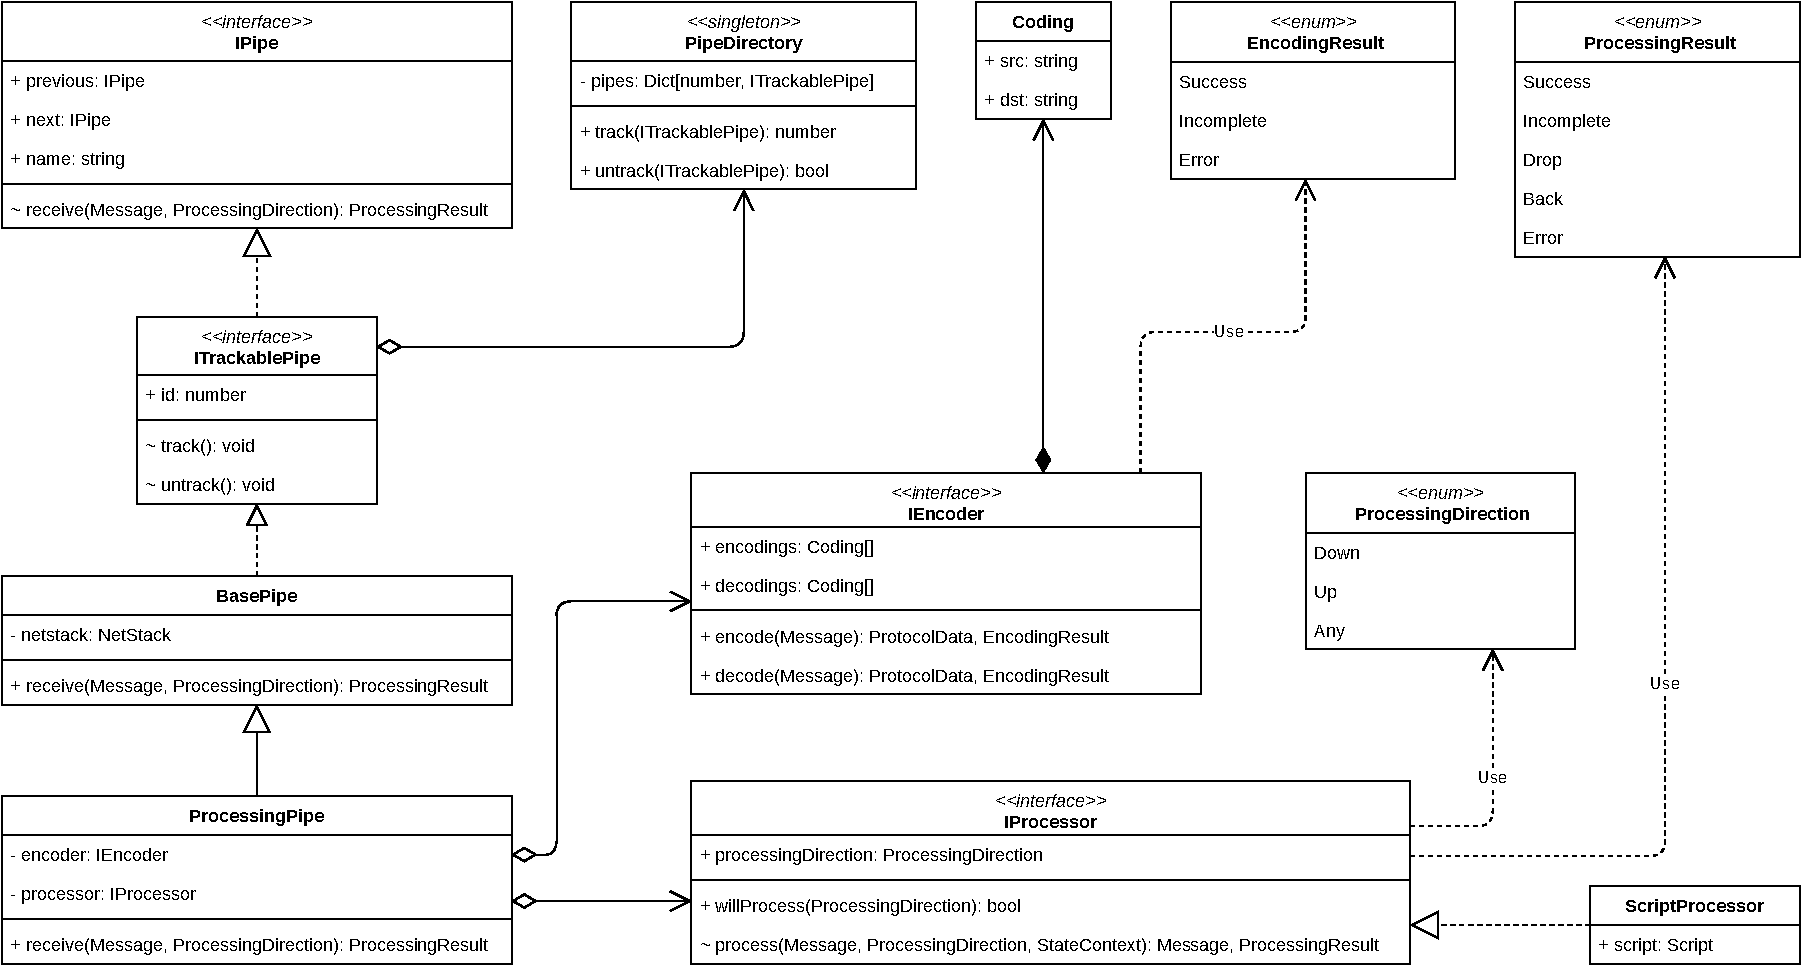
\includegraphics[width=14cm]{img/ch05/classes-2-pipes.pdf}
    \captionof{figure}{The interfaces, classes and enums used to represent pipes, their specializations and associated classes. This iteration separates \emph{BasePipes} from \emph{IEncoders} and \emph{IProcessors} so \emph{BasePipes} only implement routing of messages.}
    \label{fig:classes-2-pipes}
\end{figure}

\subsection{Pipes} Building upon the approach of routing and processing messages via pipes discussed in section \ref{sec:prototype-design}, this design concept addresses some inconsistencies of the former design and adds needed flexibility. As shown in figure \ref{fig:classes-2-pipes}\footnote{A larger printout \ref{fig:app-classes-2-pipes} can be found in the appendix.}, the \enquote{IPipe} interface is reused from the first prototype and extended by the \enquote{ITrackablePipe} interface that adds a unique identifier to pipes. This enables the application to easily locate pipes by looking up their identifiers in the \enquote{PipeDirectory}, allowing to interact with and inject messages into individual pipes directly.\\
A \enquote{BasePipe} implements the ITrackablePipe interface as well as simple routing logic for forwarding messages up and down pipelines. However, only \enquote{ProcessingPipes} actually perform any kind of operations on messages directly: they can employ \enquote{IEncoders} for (de-)serialization and \enquote{IProcessors} for transformation of messages. Contrary to the design concept of the first prototype, IEncoders need to specify which data formats they support as source and target encodings. This allows the implementation of multiple IEncoders for the same protocol that work with different source or target data formats. For example, some IEncoder may only provide decoding functionality for raw binary data into \ac{HTTP} messages with raw binary bodies while another implementation provides functionality to encode strings into \ac{HTTP} message bodies. In the first prototype's design, the very concept of filters was only vaguely described and lacked a clear and concise interface. This issue is resolved in this next iteration of the design concept:
\begin{itemize}
    \item Filters are renamed to \enquote{IProcessors} (conveying the purpose and meaning of the interface in its name).
    \item IProcessors specify a \enquote{ProcessingDirection} that determines whether messages shall be processed on their way \emph{down} or \emph{up} a pipeline or in any direction, effectively granting control over applying transformations on messages. This can be helpful when transformations shall only be applied in one direction or maybe only once in a pipeline, like replacing the contents of the body of an \ac{HTTP} message.
    \item An IProcessor can apply logic to messages in its \emph{process} method that also receives the pipeline's context. The returned \enquote{ProcessingResult} indicates success or failure of the operation or whether the IProcessor requests dropping a message or sending it back up the pipeline.
\end{itemize}
While there are many opportunities for specific implementations of the IProcessor interface, one general implementation is envisioned by the design concept: a simple \enquote{ScriptProcessor} allows penetration testers to supply scripts that are executed at runtime and allow transformation of messages. This directly fulfils the requirement \enquote{F5 Scripting}.
\begin{figure}[h]
    \centering
    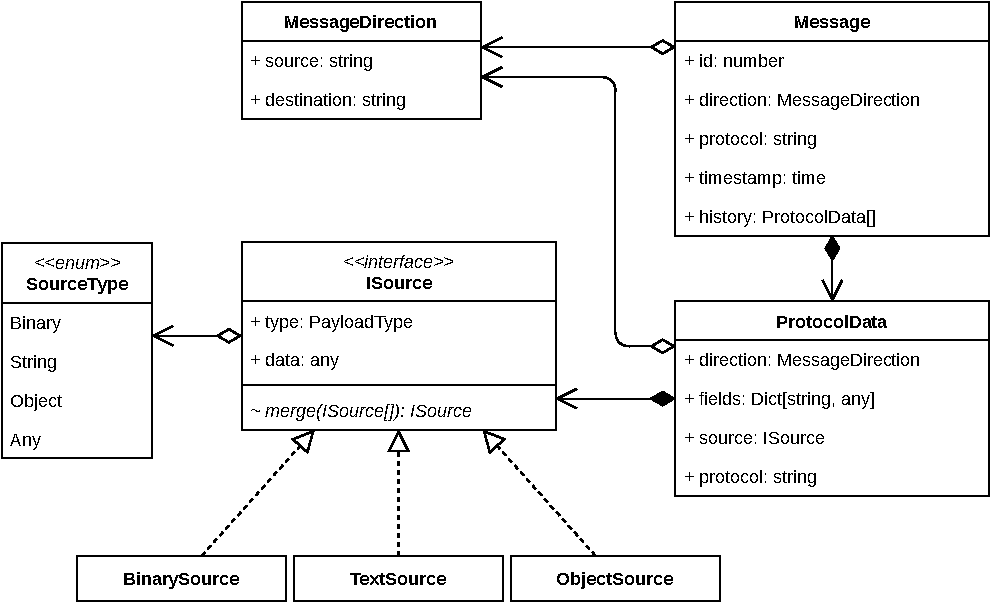
\includegraphics[width=14cm]{img/ch05/classes-4-messages.pdf}
    \captionof{figure}{The data-structures used to represent messages, their meta-data and payloads.}
    \label{fig:classes-4-messages}
\end{figure}
\subsection{Messages}
Compared to the first prototype's design, the data-structures that represent messages are mostly unchanged (as shown in figure \ref{fig:classes-4-messages}). However, during implementation and testing of the first prototype it became apparent that in some cases \enquote{historical} information about messages was required. This iteration of the design adds a list of \enquote{ProtocolData} instances to messages that specify information about the protocol, message headers and the payload (\enquote{ISource}). IProcessors and IEncoders append newly transformed or (de-)serialized ProtocolData instances to messages. So over time, a message contains records of all those operations performed on it. This information can be useful in a number of cases like serialization: when a message is deserialized (e.g. the payload of a \ac{WS} message is extracted) on its way down a pipeline, important information about the formerly encapsulating protocol is lost (such as the \ac{WS} frame's flags). When a message is serialized on its way back up a pipeline, an IEncoder would have to generate this information or try and deduce it from the message, which is not always possible. However, since it can access the messages' history and former ProtocolData, it can read the original information and use this for serialization.

\section{Design \#2: Distributed Proxy Services}
\label{sec:design-2}
The design shown in section \ref{sec:design-1} was an iteration of the design worked out for the first prototype in section \ref{sec:prototype-design} and addressed some fundamental, architectural flaws and aimed for better flexibility and more meaningful interface definitions. However, it did not address other problems that were encountered during the implementation of the first prototype: constraints in platform, framework and programming language compatibility and flexibility. As a consequence of these constraints, the proxy application needed to be developed as a monolithic application. Therefore, each extension, like additional IEncoders that added support for new protocols, was required to be implemented in the same programming language and run on the same platform and as part of the same process as the proxy application. This also effectively limited the available selection of libraries. Another potential problem of the former design concept was the tight coupling of pipes and the deeply nested structure and hierarchy of state-machines, pipes and network stacks. While this architecture allowed to implement routing messages through composition (\emph{by design}), it greatly added to the runtime complexity and made debugging the application significantly harder.
\begin{figure}[h]
    \centering
    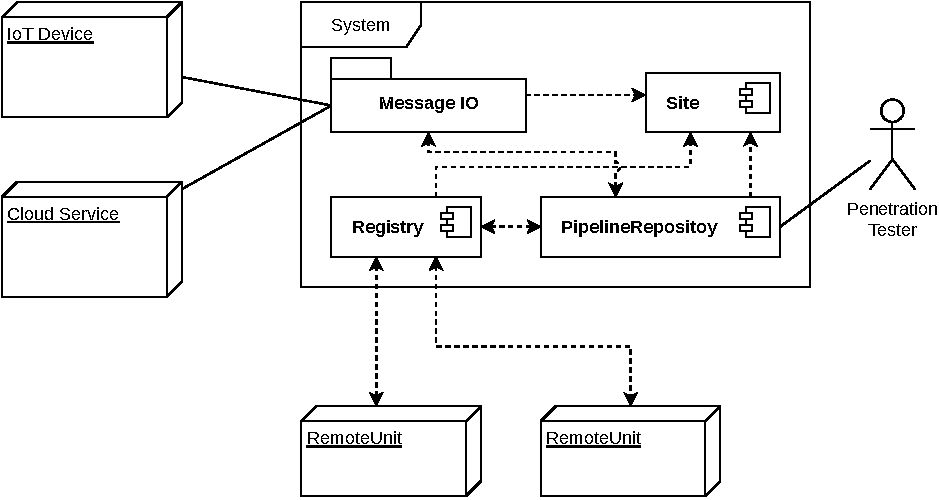
\includegraphics[width=14cm]{img/ch05/component-view2-1.pdf}
    \captionof{figure}{A component diagram showing the external systems communicating with the system and their connection to internal components.}
    \label{fig:component-view2-1}
\end{figure}
\subsection{Overview}
Another iteration of the design (shown in figure \ref{fig:component-view2-1}) was made to address these issues. While the \enquote{Message IO} and \enquote{Site} components are left unchanged, the global state-machine is replaced by the \enquote{Registry} and \enquote{PipelineRepository} components that allow for de-centralized and more controlled processing of messages.

\begin{figure}[h]
    \centering
    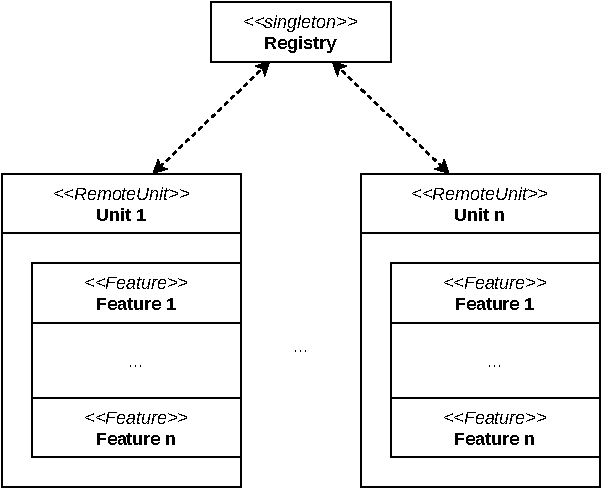
\includegraphics[width=10cm]{img/ch05/registry-remoteunit.pdf}
    \captionof{figure}{In this concept, $n$ separate \emph{Units} can be registered at a central \emph{Registry}. \emph{Units} may provide an arbitrary amount of \emph{Features}.}
    \label{fig:registry-units}
\end{figure}
\begin{figure}[ht]
    \centering
    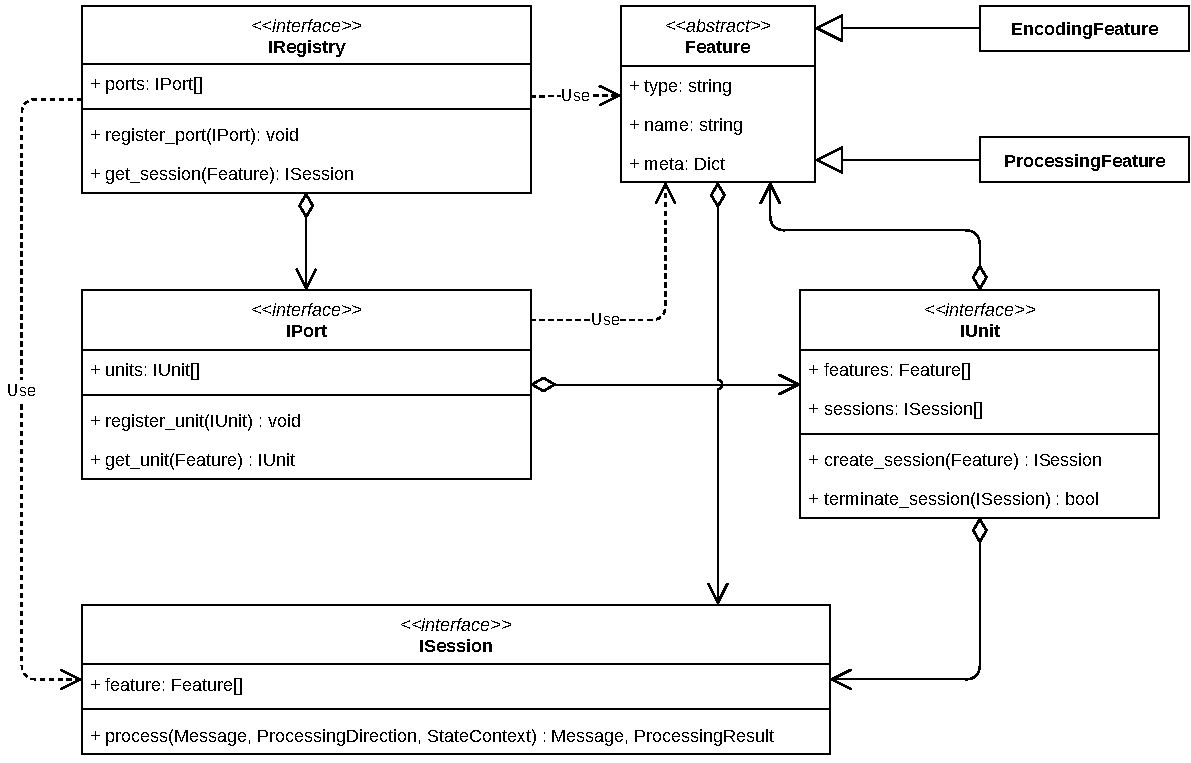
\includegraphics[width=14cm]{img/ch05/component-view2-3-registry-port-unit.pdf}
    \captionof{figure}{Visualized in this diagram, the distributed implementation and central registration of features is the core idea of the Registry and Unit components.}
    \label{fig:component-view2-3-registry-port-unit}
\end{figure}
\subsection{Registry and Units} To implement de-centralized processing of messages, a central registry is required to register remote units (shown in figure \ref{fig:registry-units}).
As can be seen in figure \ref{fig:component-view2-3-registry-port-unit}, the central registry is represented by the \enquote{IRegistry} interface that allows remote units to register themselves and allows the PipelineRepository to request sessions to units that implement requested features. Remote units can be remote machines that implement the \enquote{IPort} interface that provides a list of \enquote{IUnit} instances. An IUnit implements one or more \enquote{Features}, such as specific (de-)serialization or other processing, and effectively provides IEncoder and IProcessor functionalities. This transforms formerly direct calls to IEncoders and IProcessors to \acp{RPC}. Since IEncoders and IProcessors can be stateful, IUnits initialize them in \enquote{ISessions} for each requested feature. The IRegistry and IPort interfaces are explicitly kept rather simple and unspecific to the exact means of communication between them so that they can be implemented in various ways, making use of various \ac{IPC} techniques.\\
Also, to transmit data between the proxy application and its remote units, this data needs to be (de-)serialized and a format for serialization has to be chosen.

\subsection{PipelineRepository} The PipelineRepository component holds information about all configured pipelines (that is a flattened representation of the hierarchically configured state-machines and network stacks) and their contexts. This allows to remove the pipes from the software architecture, providing better traceability of messages throughout the system and makes debugging the high-level application logic more accessible. Also, organizing network stacks and state-machines in one central place encourages creation of means to interface with these mechanisms such as \ac{REST}-\acp{API} that let penetration testers inspect the message queue and ongoing processes.

\subsection{State of the Design Concept}\label{sec:design-2-state} This design concept promises to solve severe issues of the previous design iteration shown in section \ref{sec:design-1} and already defines some very high-level components. However, due to time constraints some components' designs were not  finished and require further work on specifics. For this, certain questions need to be answered and translated into the design:
\begin{itemize}
    \item \textbf{PipelineRepository:} How exactly is the hierarchy of state-machines and network stacks flattened? How is this flattened hierarchy represented in data-structures? How are instances of individual state-machines and network stacks initialized and organized for individual gateway-connections?
    \item \textbf{ISession:} How is information relevant to IEncoder and IProcessor instances (such as ScriptProcessors' Script instances) passed to remote units?
    \item \textbf{IRegistry/IPort:} How exactly are \acp{RPC} performed? Are there mature and appropriate frameworks that provide \acp{RPC} implementations?
\end{itemize}


\subsection{Comparison of Both Designs}
\label{sec:design-comparison}
Both design concepts discussed in the previous sections, the monolithic and the distributed concept, promise to solve specific problems. The following paragraphs compare both concepts on the base of a set of core design aspects:
\paragraph{Software architecture}
The monolithic concept suggests a centralized and self-contained design that combines the high-level business logic of a proxy-application with low-level tasks such as (de-)serialization of various protocols. It is designed to be run on a single machine.\\
In contrast to this, the distributed concept separates the high-level business logic (like routing messages) and low-level tasks as part of a client-server model: the high-level logic is implemented in the central proxy server while low-level tasks are isolated into separate remote services. These services can either be run on the same machine the proxy server runs on or on external machines. Through dynamic creation and registration of remote service instances, this concept also implements scalability. Since there is no restrictions to the programming languages, platforms or frameworks used by remote services, the concept also embraces platform compatibility.
\paragraph{Complexity}
The reliance on deeply nested data-structures has a high impact on the complexity of the monolithic concept at runtime. This makes debugging an implementation of this concept significantly harder and more time-consuming. However, adding new extensions to this concept becomes a comparatively easier task as integration of such new extensions only takes place on a source-code level.\\
As opposed to this, the distributed approach simplifies the high-level tasks such as routing messages by introducing distributed components that allow traceability and thus establish transparency. The offloading of protocol implementations into logical units that are accessed via \ac{IPC} however contribute to a more challenging deployment of the application. Also, due to their distributed nature, debugging these remote units can introduce further problems (e.g. connection losses and high latencies) and requires a more sophisticated and complex testing environment than the monolithic concept.

\paragraph{Maturity}
Some of the core components of the monolithic concept were already tested and proven by the first prototype. For instance, linked pipes proved to be an effective means to route and process messages up and down a processing pipeline. However, due to time-constraints, other core concepts such as the state-machines could not be tested. Regarding completeness, it is noteworthy that this concept's interfaces are well-defined.\\
Contrary to this, the distributed concept is not finished and requires further work to clear up a number of essential questions before it can be completed. Also, the previously proven effective idea of using pipes for routing and processing is removed in the distributed approach. This denies the approach any effectiveness acquired through previous design iterations.